\documentclass[12pt,a4]{article}
\usepackage[greek,english]{babel}
\usepackage{graphicx}
\graphicspath{ {./images/} }
\usepackage{hyperref}

\textwidth      6.5in
\textheight     8.7in
\oddsidemargin  0.0cm
\evensidemargin 0.0cm
\parindent      0pt
\topmargin      0.1in
\headsep        20pt

\parskip        10pt
\parindent      0pt

\newcommand{\gr}{\greektext}
\newcommand{\la}{\latintext}

\newcommand{\ilcode}[1]{\textcolor[RGB]{160, 110, 220}{#1}}

\begin{document}

\begin{titlepage}
	\begin{center}
		% Title.
		\vspace*{1cm}
		\Huge
		\textbf{{\la Intro to Git}}
		
		% Subtitle.
		\vspace{0.5cm}
		\LARGE
		{\sf \la Workshop}

		% Participants in alphabetical order.
		\vspace{1.5cm}
		\normalsize
		\textbf{Κιορπελίδης Πλάτων}\\
		\textbf{Μπαζιότης Στέφανος}

		\vfill
		
		%\includegraphics[width=0.4\textwidth]{uni-logo}
		\scalebox{2}{%
			
\includegraphics[width=0.4\textwidth]{acmuoa}}

		\LARGE
		{\sf \la University of Athens}\\
		{\sf \la ACM UoA Student Chapter}

		% Some cool coffee stains.
		\cofeAm{0.08}{0.8}{120}{200}{-200}
		\cofeAm{0.06}{0.8}{240}{150}{-140}
	\end{center}
\end{titlepage}


\section{Introduction}
\subsection{Git \& Version Control}
{\sf -- \emph{The Problem}:}
Many people’s version-control method of choice is to copy files into another
directory. We create copies of the project and name them to \emph{project v2},
\emph{project v3}, etc. This approach is very common because it is so simple,
but it is also incredibly error prone. It is easy to forget which directory
you’re in and accidentally write to the wrong file or copy over files you don’t
mean to, delete code that may be useful later -- whenever you have the entire
history of the project in a single place, you risk losing everything. In
addition, it clutters up the workspace and gives vertigo to anyone browsing it.

We also want to collaborate with other developers. We could keep the codebase
under a server but what about server failures. If the server goes down for an
hour, then during that hour nobody can collaborate at all or save versioned
changes to anything they're working on. If the hard disk the central database is
on becomes corrupted, and proper backups haven’t been kept, you lose absolutely
everything -- the entire history of the project except whatever single snapshots
people happen to have on their local machines.

{\sf -- \emph{The Solution}:} This is where Distributed Version Control Systems
step in, like Git. In such systems, clients don’t just check out the latest
snapshot of the files; rather, they fully mirror the repository, including its
full history. Thus, if any server dies, and these systems were collaborating via
that server, any of the client repositories can be copied back up to the server
to restore it. Every clone is really a full backup of all the data.

\textcolor[RGB]{220,220,220}{\rule{\linewidth}{0.8pt}}

{\sf Version Control:} It's is a system that records changes to a file or a set
of files over time so that you can recall specific versions later.

{\sf Distributed Version Control System:} Clients fully mirror the remote
repository, including it's history. Remote repository is stored in a server.
Full copy of the code is present in all the developers' computers.

Popularity of Git (2010 vs 2019):
\vspace*{-5pt}
\begin{itemize}
\item 2010: 26,485 repositories (11.3\% of total)
\item 2019: 913,378 repositories (70\% of total)
\end{itemize}

{\sf Server example:} GitHub. GitHub is the single largest hosting server for
Git repositories with a web front end. It offers all of the distributed version
control and source code management (SCM) functionality of Git as well as adding
its own features. It provides access control (users) and several collaboration
features such as bug tracking, feature requests, task management, and wikis for
every project. A large percentage of all Git repositories are hosted on GitHub,
and many open-source projects use it for Git hosting, issue tracking, code
review, and other things. So while it’s not a direct part of the Git open source
project, there’s a good chance that you’ll want or need to interact with GitHub
at some point while using Git professionally.

\subsection{Concept of Git \& Early days}
Git follows the unix philosophy. The Unix philosophy emphasizes building simple,
short, clear, modular, and extensible code that can be easily maintained and
repurposed by developers other than its creators. The Unix philosophy favors
composability as opposed to monolithic design.

In it's early days git consisted of simple, atomic executables. Such programs
weren't enough to be useful on their own, but a combination of those, usually in
shell scripts, composed more complex functionality like \ilcode{\bf git add}.
Probably it's the reason, after so many developement cycles, still considered a
complex and difficult tool.

It was created by Linus Torvalds to help maintain Linux. As more people were
sending in patches and the current workflow didn't scale, Linus created a new
VCS as he didn't like existing ones. He named it git -- the stupid content
tracker or the information manager from hell.

\subsubsection{Meaning of Git}
\vspace*{-10pt}
\emph{Copied from the first git commit written by Linus Torvalds.}

"git" can mean anything, depending on your mood.
\begin{itemize}
\vspace*{-10pt}
\item Random three-letter combination that is pronounceable, and not actually
	used by any common UNIX command. The fact that it is a mispronounciation of
	"get" may or may not be relevant.
\vspace*{-3pt}
\item Stupid. Contemptible and despicable. Simple. Take your pick from the
	dictionary of slang.
\vspace*{-3pt}
\item "global information tracker": you're in a good mood, and it actually
   works for you. Angels sing, and a light suddenly fills the room.
\vspace*{-3pt}
\item "goddamn idiotic truckload of sh*t": when it breaks.
\vspace*{-10pt}
\end{itemize}

This is a stupid (but extremely fast) directory content manager. It doesn't do
a whole lot, but what it does do is track directory contents efficiently.

\subsection{Modern Git}
Initially git wasn't developed for the novice user. Nowdays it's a lot
friendlier and easier to get into as it comes with a lot of build-in commands,
wrappers and complexity abstractions. These commands internally use the old,
enhanced, but still atomic executables. There are GUIs developed for the GUI
lovers or non-technical people and it's supported with plugins by various text
editors and IDEs. These changes and features make for an easier, faster and
streamlined collaboration between developers, who follow various local and
online workflows.

\section{Installing Git}
Before you start using Git, you have to make it available on your computer. Even
if it’s already installed, it’s probably a good idea to update to the latest
version. You can either install it as a package or via another installer, or
download the source code and compile it yourself.

{\sf -- Linux (Debian, Ubuntu):} \ilcode{sudo apt-get install git-all}

{\sf -- Max:} Run \ilcode{git -{}-version}. If you don’t have it installed
already, it will prompt you to install.

{\sf -- Windows:} Download from \url{https://git-scm.com/download/win}.

\section{Working locally}
\subsection{Initializing Git (git init)}
If you have a project directory that is currently not under version control and
you want to start controlling it with Git, you first need to go to that
project’s directory \ilcode{cd /home/user/my\_project} and type \ilcode{git
init}. This creates a new subdirectory named .git that contains all of your
necessary repository files -- a Git repository skeleton. A project that is under
Git is called "repository" or "repo". At this point, nothing in your project is
tracked yet.

In order to start tracking our changes and as a result our project we need to
inform Git about our identity. This is important because every Git commit uses
this information, and it’s immutably baked into the commits you start creating:

\hspace*{1cm}
\ilcode{\$ git config --global user.name "John Doe"}\\
\hspace*{1cm}
\ilcode{\$ git config --global user.email johndoe@example.com}

{\sf NOTE:} \ilcode{-{}- global} sets your name and email across Git projects.
If you want to have a different identity for different projects run the above
instructions without \ilcode{-{}- global} flag. You can check your settings with
\ilcode{git config -{}- list}.

\begin{center}
\scalebox{2}{%
	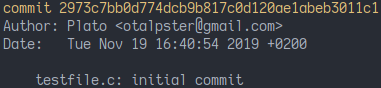
\includegraphics[width=0.4\textwidth]{gitlog}}
\end{center}

{\sf -- \emph{Exercise}:} Open your laptops! Open a terminal and create a
directory. Inside the new directory run \ilcode{git init}. Then run \ilcode{ls
-la} and notice the hidden directory \ilcode{.git}.

\subsection{The three stages}
\begin{center}
\scalebox{2.5}{%
	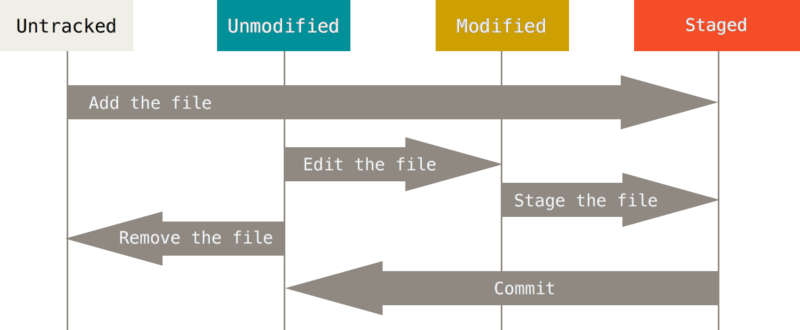
\includegraphics[width=0.4\textwidth]{lifecycle}}
\end{center}

Each file in your working directory can be in one of two states: tracked or
untracked. Tracked files are files that were in the last snapshot; they can be
unmodified, modified, or staged. In short, tracked files are files that Git
knows about.

Untracked files are everything else -- any files in your working directory that
were not in your last snapshot and are not in your staging area. When you first
create a file it will be untracked because Git does not track it yet.

As you edit files, Git sees them as modified, because you’ve changed them since
your last commit. As you work, you selectively stage these modified files and
then commit all those staged changes, and the cycle repeats.

\subsection{Checking the status of your file (git status)}
The tool you use to determine which files are in which state is the \ilcode{git
status} command.

{\sf -- \emph{Exercise}:} Run \ilcode{git status}. Create a new file
\ilcode{touch testfile}. Run \ilcode{git status} again. The new file should
appear as \ilcode{untracked}.

\subsection{Staging changes (git add)}
\ilcode{git add} moves changes to the staging area. Changes to Git means
anything it does not know, new files or modified ones. The staging area is where
we are cooking the contents of our next snapshot.

{\sf -- \emph{Exercise}:} Let's track our new file. Run \ilcode{git add}. See
that our new file is in the staging area with \ilcode{git status}. Now our
untracked file is cooking for the next snapshot! When Git records the current
staging area and creates a new snapshot our untracked file will become tracked.
Until then it's just staged.

{\sf -- \emph{Exercise}:} Open your editor of choice and change the testfile.
Add some random letters. Run \ilcode{git status}. Notice that the testfile is
listed as both staged and unstaged.

How is this possible? It turns out that Git stages a file exactly as it is when
you run \ilcode{git add}. If you record a new snapshot now, the version of
testfile as it was when you last ran \ilcode{git add} is how it will go into the
snapshot, not the version of the file as it looks in your working directory. If
you modify a file after you run \ilcode{git add}, you have to run \ilcode{git
add} again to stage the latest version of the file.

\subsection{Viewing your staged and unstaged changes (git diff)}
Sometimes, \ilcode{git status} command is too vague. You want to know exactly
what you changed, not just which files were changed. To achive this you use the
\ilcode{git diff} command. You most often use it to answer these two questions:
What have you changed but not yet staged? What have you staged that you are
about to commit? \ilcode{git status} answer these questions by listing the file
names, \ilcode{git diff} shows you the exact lines added and removed -- the
patch, as it were.

To see changes you've made that you haven't yet staged, type \ilcode{git diff}.
That command compares what is in your working directory with what is in your
staging area.

To see what you’ve staged that will go into your next commit, you can use
\ilcode{git diff --staged}. This command compares your staged changes to your
last commit.

{\sf -- \emph{Exercise}:} View your changes. Run \ilcode{git diff}. Run
\ilcode{git diff --cached}. Notice the + and - characters. What do they mean?
+, - describes the added and removed lines respectively.

It’s important to note that \ilcode{git diff} by itself doesn’t show all changes
made since your last commit -- only changes that are still unstaged. If you’ve
staged all of your changes, \ilcode{git diff} will give you no output. You will
need to run \ilcode{git diff} and \ilcode{git diff --staged} to show all changes
made since your last commit, staged and unstaged.

\ilcode{git status} can reproduce the above behaviour by running internally and
formatting the output of \ilcode{git diff} and \ilcode{git diff --staged} with
the flag \ilcode{git status -v}/\ilcode{-vv}. The \ilcode{-v} flag, in addition
to the output of \ilcode{git status}, will also show the actual changes that are
staged to be committed, like \ilcode{git diff -{}-cached}. The \ilcode{-vv}
flag, in addition to the output of \ilcode{git status -v}, will also show the
changes that have not yet been staged, like \ilcode{git diff}.

{\sf -- \emph{Exercise}:} View your changes. But this time run \ilcode{git
status -v}. Run \ilcode{git status -vv}. See the difference and the similarity
with \ilcode{git diff}/\ilcode{git diff -{}-cached}?

\subsection{Snapshoting/Committing your changes (git commit)}
Now that your staging area is set up the way you want it, you can commit your
changes. Remember that anything that is still unstaged -- any files you have
created or modified that you haven’t run \ilcode{git add} on since you edited
them -- won’t go into this commit. They will stay as modified files on your
disk. So you’re ready to commit your changes. The simplest way to commit is to
type \ilcode{git commit}.

Each commit consists of the {\bf commit message} and a {\bf body}. It's a common
practise to write commit messages with up to 50 characters. Commit messages are
used for a brief but descriptive explanation about what changes you are
committing. The body should provide a meaningful commit message, for example:
\begin{itemize}
\item Explains the problem the change tries to solve, i.e. what is wrong with
	the current code without the change.
\item Justifies the way the change solves the problem, i.e. why the result with
	the change is better.
\item Alternate solutions considered but discarded, if any.
\end{itemize}
If your description starts to get too long, that’s a sign that you probably need
to split up your commit to finer grained pieces. Descriptions that summarize the
point in the subject well, and describe the motivation for the change, the
approach taken by the change, and if relevant how this differs substantially
from the prior version, are all good things to have.

{\sf -- \emph{Exercise}:} Commit your changes. Run \ilcode{git commit}. Doing so
will launch the default editor with the output of \ilcode{git status} commented
out. The first line is the commit message. Leave a blank line and write a short
description.

{\sf -- \emph{Exercise}:} Stage your changes. Run \ilcode{git add}. Now commit
them. Sometimes you forget what you are committing and need even more explicit
reminder than the commented out \ilcode{git status}. Run \ilcode{git commit -v}.
Doing so also puts the diff of your change in the editor so you can see exactly
what changes you're committing. Save and exit the editor to create your commit.

Alternatively, you can type your commit message inline with the commit command
by specifying it after a -m flag, like this:

\hspace*{1cm}
\ilcode{\$ git commit -m "Story 182: Fix benchmarks for speed}

Remember that the commit records the snapshot you set up in your staging area.
Anything you didn’t stage is still sitting there modified; you can do another
commit to add it to your history. Every time you perform a commit, you’re
recording a snapshot of your project that you can revert to or compare to later.

\subsection{Viewing the commit history (git log)}
After you have created several commits, or if you collaborate with others and
they made changes (more later), you’ll probably want to look back to see what
has happened. The most basic and powerful tool to do this is the \ilcode{git
log} command.

By default, with no arguments, \ilcode{git log} lists the commits made in that
repository in reverse chronological order; that is, the most recent commits show
up first. As you can see, this command lists each commit with its SHA-1
checksum, the author’s name and email, the date written, and the commit message.

A huge number and variety of options to the git log command are available to
show you exactly what you’re looking for. Here, we’ll show you some of the most
useful.

{\sf -- \emph{Exercise}:} Run \ilcode{git log -{}-one-line}. One line per commit.

{\sf -- \emph{Exercise}:} Run \ilcode{git log -n}. Show the last $n$ commits.

{\sf -- \emph{Exercise}:} Run \ilcode{git log -p}. Show the changes introduced.

{\sf -- \emph{Exercise}:} Run \ilcode{git log -{}-stat}. Abbreviated commit stats.

\subsection{Undoing staged and modified changes}
At any stage, you may want to undo something. Here, we’ll review a few basic
tools for undoing changes that you’ve made. Be careful, because you can’t always
undo some of these undos. This is one of the few areas in Git where you may lose
some work if you do it wrong.

\subsubsection{Unstaging a Staged File}
You made a mistake and ran \ilcode{git add} against a file which you don't want
to commit yet. How can you unstage it? The \ilcode{git status} command reminds
you.

{\sf -- \emph{Exercise}:} Make a very simple change. Run \ilcode{git add}. Now
run \ilcode{git status}. Run \ilcode{git reset HEAD testfile} to unstage. The
command is a bit strange, but it works. The testfile file is modified but once
again unstaged.

{\sf NOTE:} \ilcode{git reset} can be a dangerous command. However, in the
scenario described above, the file in your working directory wasn't touched, so
it’s relatively safe.

\subsubsection{Unmodifying a Modified File}
What if you realize that you don’t want to keep the changes you made to a file?
How can you easily unmodify it -- revert it back to what it looked like when you
last committed? Luckily, \ilcode{git status} tells you how to do that, too.

{\sf -- \emph{Exercise}:} Run \ilcode{git status}. Run \ilcode{git checkout -{}-
testfile}. You can see that the changes have been reverted.

{\sf NOTE:} It’s important to understand that \ilcode{git checkout -{}- <file>}
is a dangerous command. Any local changes you made to that file are gone -- Git
just replaced that file with the most recently-committed version. Don’t ever use
this command unless you absolutely know that you don’t want those unsaved local
changes.

Know that anything that is committed in Git can almost always be recovered. Even
commits that were deleted or commits that were overwritten/modified can be
recovered. However, anything you lose that was never committed is likely never
to be seen again.

\end{document}
